\section{Datasets}

\subsection{Obtaining a high resolution dataset}
    
    
Super-resolution is inherently a supervised learning task that needs the availability of high-resolution (HR) data. In scenarios where HR data from sources like FOREST-2 is unavailable, an alternative is to generate synthetic images from external missions, with similar characteristics as the FOREST-2 mission but with a superior resolution.

\subsubsection{The ECOSTRESS mission}

The NASA's ECOsystem Spaceborne Thermal Radiometer Experiment on Space Station (ECOSTRESS) mission is designed to provide new insights the effects of the Earth's climate dynamics \cite{ECOSTRESS2023}, with focus on the following scientific objectives:

\begin{enumerate}
    \item Identify the critical thresholds of water use and water stress in key climate-sensitive biomes, typically by observing the transition zones between biomes.
    \item Identify when plants stop taking up water over the course of a day.
    \item Improve the accuracy of drought estimates based on agricultural water use in the continental United States. 
\end{enumerate}

ECOSTRESS employs thermal infrared radiometers, specifically Prototype HyspIRI Thermal Infrared Radiometer \cite{PhyTIR2023} to measure the radiation emitted from the Earth's surface. It provides a spatial resolution of 69 meters with a temperature sensitivity of a few tenths of a degree \cite{ECOSTRESS2023}.  The swath size is 400x400 km. The detector separates the energy from five different wavelengths using filters attached to the detector, producing five separate image layers for each scene. The pixels represent the intensity of thermal infrared radiation emitted by the Earth's surface at each wavelength. The mission has a 4-day diurnal repeat cycle.

In the spatial domain, ECOSTRESS constitutes an excellent candidate for generating synthetic HR images, as it's resolution constitutes approximately a x3 increase compared to FOREST-2. 

In the spectral domain, it is important to confirm overlap between the missions bands. Given the narrower ECOSTRESS bands, the strategy will be averaging the radiances to align the spectral properties.
Fig. \ref{fig:5-wavelength-comparison} shows this spectral band comparison.
In the case of the LWIR1 FOREST band, the overlap is significant with the first three ECOSTRESS bands.
Althouth the overlap is less pronounced in the LWIR2 band, the radiation spectrum of black-bodies at prevalent surface temperatures suggest the feasibility of constructing a synthetic LWIR2 from the last two ECOSTRESS bands.

While FOREST's temporal resolution exceeds that of ECOSTRESS, allowing for the monitoring of new processes, this aspect is not the primary focus of the current study and will not be taken into account.



\begin{figure}[H]
    \centering
    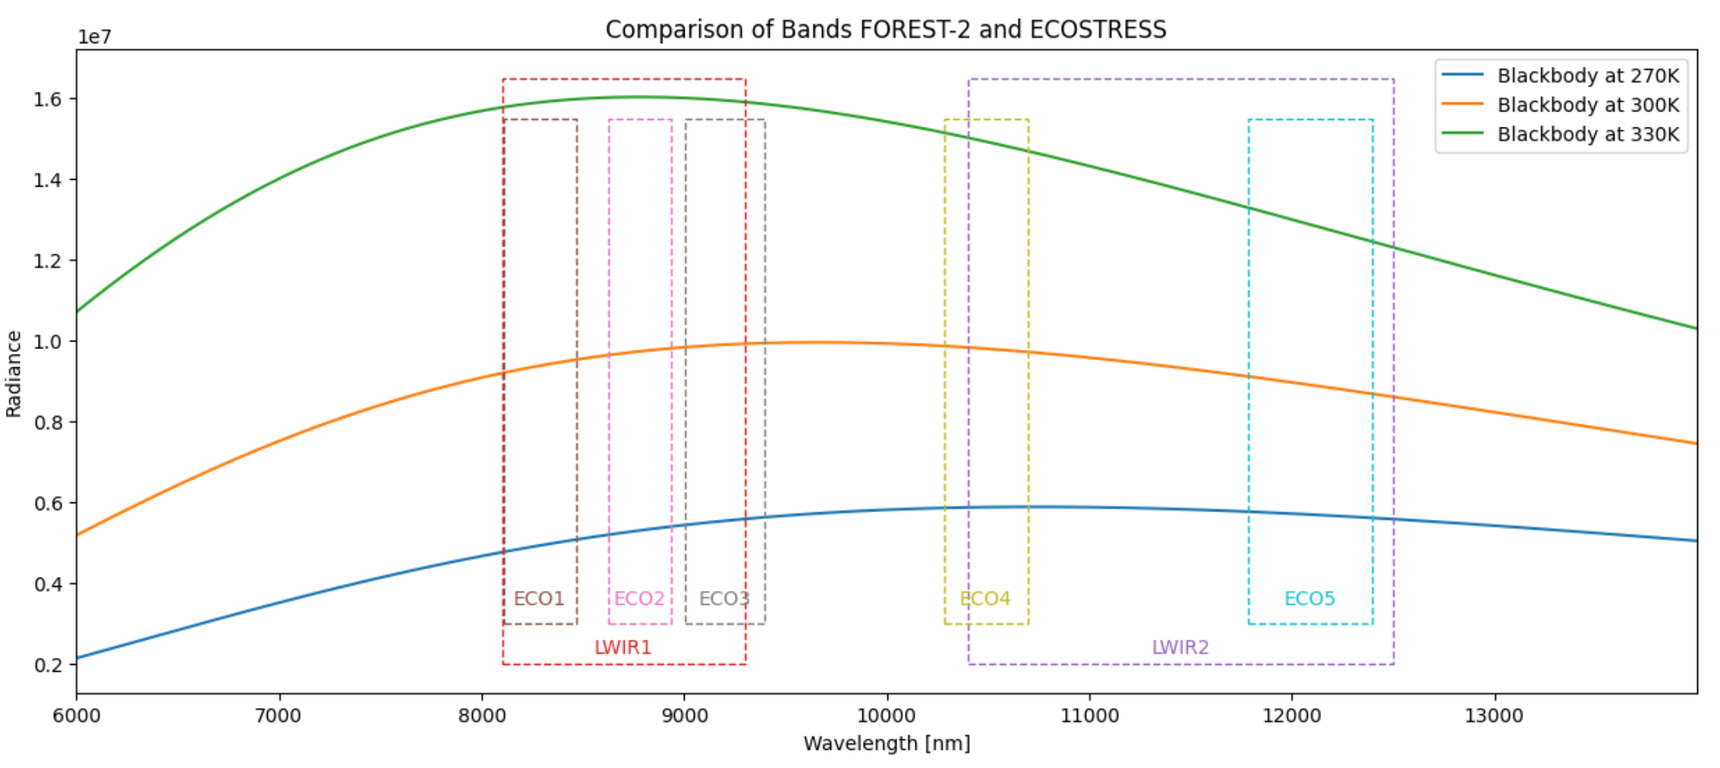
\includegraphics[width=\linewidth]{Includes/5-wavelength-comparison.png}
    \caption{Wavelengths of the sensors in Ecostress and Forest satellites. The radiation spectrum of black-bodies at different temperatures are included for comparison.}
    \label{fig:5-wavelength-comparison}
\end{figure}

\subsubsection{Accessing ECOSTRESS Scenes}
    ECOSTRESS imagery is available via NASA's Application for Extracting and Exploring Analysis Ready Samples (AppEEARS) \cite{AppEEARS2023}. This tool allows the request of area samples via vector poligons. Using the product's API \cite{AppEEARSAPI2023}, Level 1 Mapped Radiance scenes of size 200x200 km  with center on the locations provided in Fig. \ref{fig:5-wavelength-comparison} were programmatically requested. Due to satellite hardware anomalies, certain spectral bands experienced acquisition gaps, needing a careful selection of date ranges to ensure the availability of all five bands \cite{ECO1BMAPRAD2023}.

   \begin{table}[h!]
        \centering
        \begin{tabular}{|l|l|}
        \hline
        Area     & 200 x 200 km                                                                              \\ \hline
        Products & \begin{tabular}[c]{@{}l@{}}Mapped Radiance (5 bands)\\ Quality (5 Bands)\end{tabular}     \\ \hline
        Dates    & \begin{tabular}[c]{@{}l@{}}2018/08/20 - 2019/03/04\\ 2023/05/01 - 2023/08/15\end{tabular} \\ \hline
        \end{tabular}
        \caption{Requests configuration}
        \label{tab:5-scenes-characteristics}
    \end{table}

    \begin{figure}[h!]
        \centering
        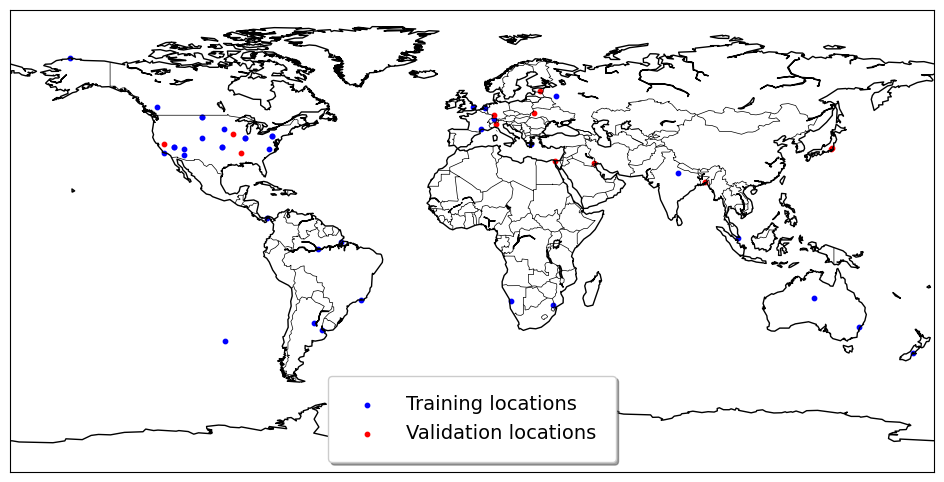
\includegraphics[width=\linewidth]{Includes/5-ecostress-map-location.png}
        \caption{Location of the samples taken from ecostress.}
        \label{fig:5-ecostress-map-location}
    \end{figure}

\subsubsection{Selecting the best scenes}

The AppEEARS platform returns multiple scenes that correspond to the specified area sample within the requested timeframe. This includes 5 mapped radiance measurements alongside their corresponding Quality Assurance (QA) bands. Additionally, a CSV file is provided, detailing quality statistics  for each scene. The interface returns any scene that overlaps with the requested area. For that reason, some GeoTIFFs may be significantly smaller than others, with variances up to 90\%. Moreover, an important number of these GeoTIFFs may contain a high percentage of bad quality pixels, rendering them unsuitable for model training. Furthermore, as highlighted in the ECOSTRESS frequently asked questions \cite{ecostress_faq}, the accuracy of radiance measurements is highly dependent on clear sky conditions; cloudy scenes typically yield negligible radiance emissions.

The dataset includes several GeoTIFFs for each scene. Downloading the entirety of this dataset is impractical due to its huge size.  
From the 50 scenes, each one is potentially replicated over 20 times over the 10 months request window.
Such a dataset, given its magnitude, cannot be used for model training with the available hardware resources.
Therefore, a procedure is developed to identify and select the most appropriate scene for each month, based on a predefined set of criteria:

\begin{enumerate}
\item Scenes should have a low proportion of bad quality pixels.
\item Scenes should have a considerable size so that many crops can be taken from it.
\item As clouds imply low radiance values, clear sky scenes will have high radiance values.
\end{enumerate}


The procedure to get the best scene for each month is detailed below: 

\begin{algorithm}
\caption{Process applied to the scenes returned from one area request.}
\begin{algorithmic}[1]

\State \textbf{QA statistics:}
\State Get the average proportion of good pixels $p_{gp}$ for the 5 radiances of the scene.
\State Discard scenes where $p_{gp} < 60 $ .

\State \textbf{Scene Statistics:}
\State Get the biggest scene of each month.
\State Calculate the proportion between the size each scene and the biggest of the month.
\State Discard images which size proportion is smaller than 0.2.
\State Calculate the median of the radiance values of the scene.
\State \textbf{Selecting the scene of the month:}
\State Merge the QA statistics and the Scene statistics.
\State For each month, get the 3 scenes with the greatest $p_{gp}$.
\State Select the scene that has the greatest median radiance value.
\end{algorithmic}
\end{algorithm}

Applying this procedure, a dataset comprised of 5031 scenes taken from 50 area requests is reduced to 379 scenes.

\subsubsection{Data Processing}

In order to be able to use the data in a super-resolution algorithm, a set of processing steps must be performed on it.

The diagram in Fig. \ref{fig:5-data_processing_flow_chart} displays the processing pipeline. The input are the 5 Mapped radiance and their respective quality bands.

Mapped radiances 1,2 and 3 are averaged to form the LWIR1 synthetic FOREST, mapped radiances 4 and 5 are averaged to form the LWIR2 synthetic FOREST. If any of the bands are missing, the corresponding LWIR synthetic forest is discarded. 

The fill values in the mapped radiances and the data quality classes are used to create a binary mask for each spectral band. If a pixel is considered problematic, it is marked as a 1 in the binary mask. The QA band for a synthetic FOREST LWIR band is built using an OR operation on the corresponding ECOSTRESS spectral involved in it's construction. After being constructed, both the synthetic LWIR and the corresponding QA band are reprojected to the best utm epsg code, based on the latitude and longitude of the scene.

\begin{table}[h!]
    \centering
    
    \label{tab:quality_classes}
    \begin{tabular}{cl}
        \toprule
        \textbf{Value} & \textbf{Description}                \\
        \midrule
        \multicolumn{2}{c}{Fill Value Classes}                \\
        -9997          & Pixel not seen                       \\
        -9998          & Missing data due to striping (not filled in) \\
        -9999          & Missing/bad data                     \\
        \midrule
        \multicolumn{2}{c}{Data Quality Classes}              \\
        0              & Good                                 \\
        1              & Missing stripe data, filled in       \\
        2              & Missing stripe data, not filled in   \\
        3              & Missing/bad data                     \\
        4              & Not seen                             \\
        \bottomrule
    \end{tabular}
    \caption{Fill Value and Data Quality Classes}
\end{table}

The synthetic LWIR are not suitable for the super-resolution task yet.
They are too big to be kept in memory, and not all their values are of good quality.
For that reason, for each scene, a number of random crops of size 264x264 pixels are taken.
The random crop processor pipeline is displayed in Fig. \ref{fig:5-random_crop_processor}.
It is an iterative process where at each stage, crops that do not comply with the quality considerations ( all pixels are of good quality and no stripe noise was detected) are discarded until the target number of crops per scene is achieved.
Additionally, the Affine Transformation is translated so that the images can be georeferenced.


\begin{figure}[H]
    \centering
    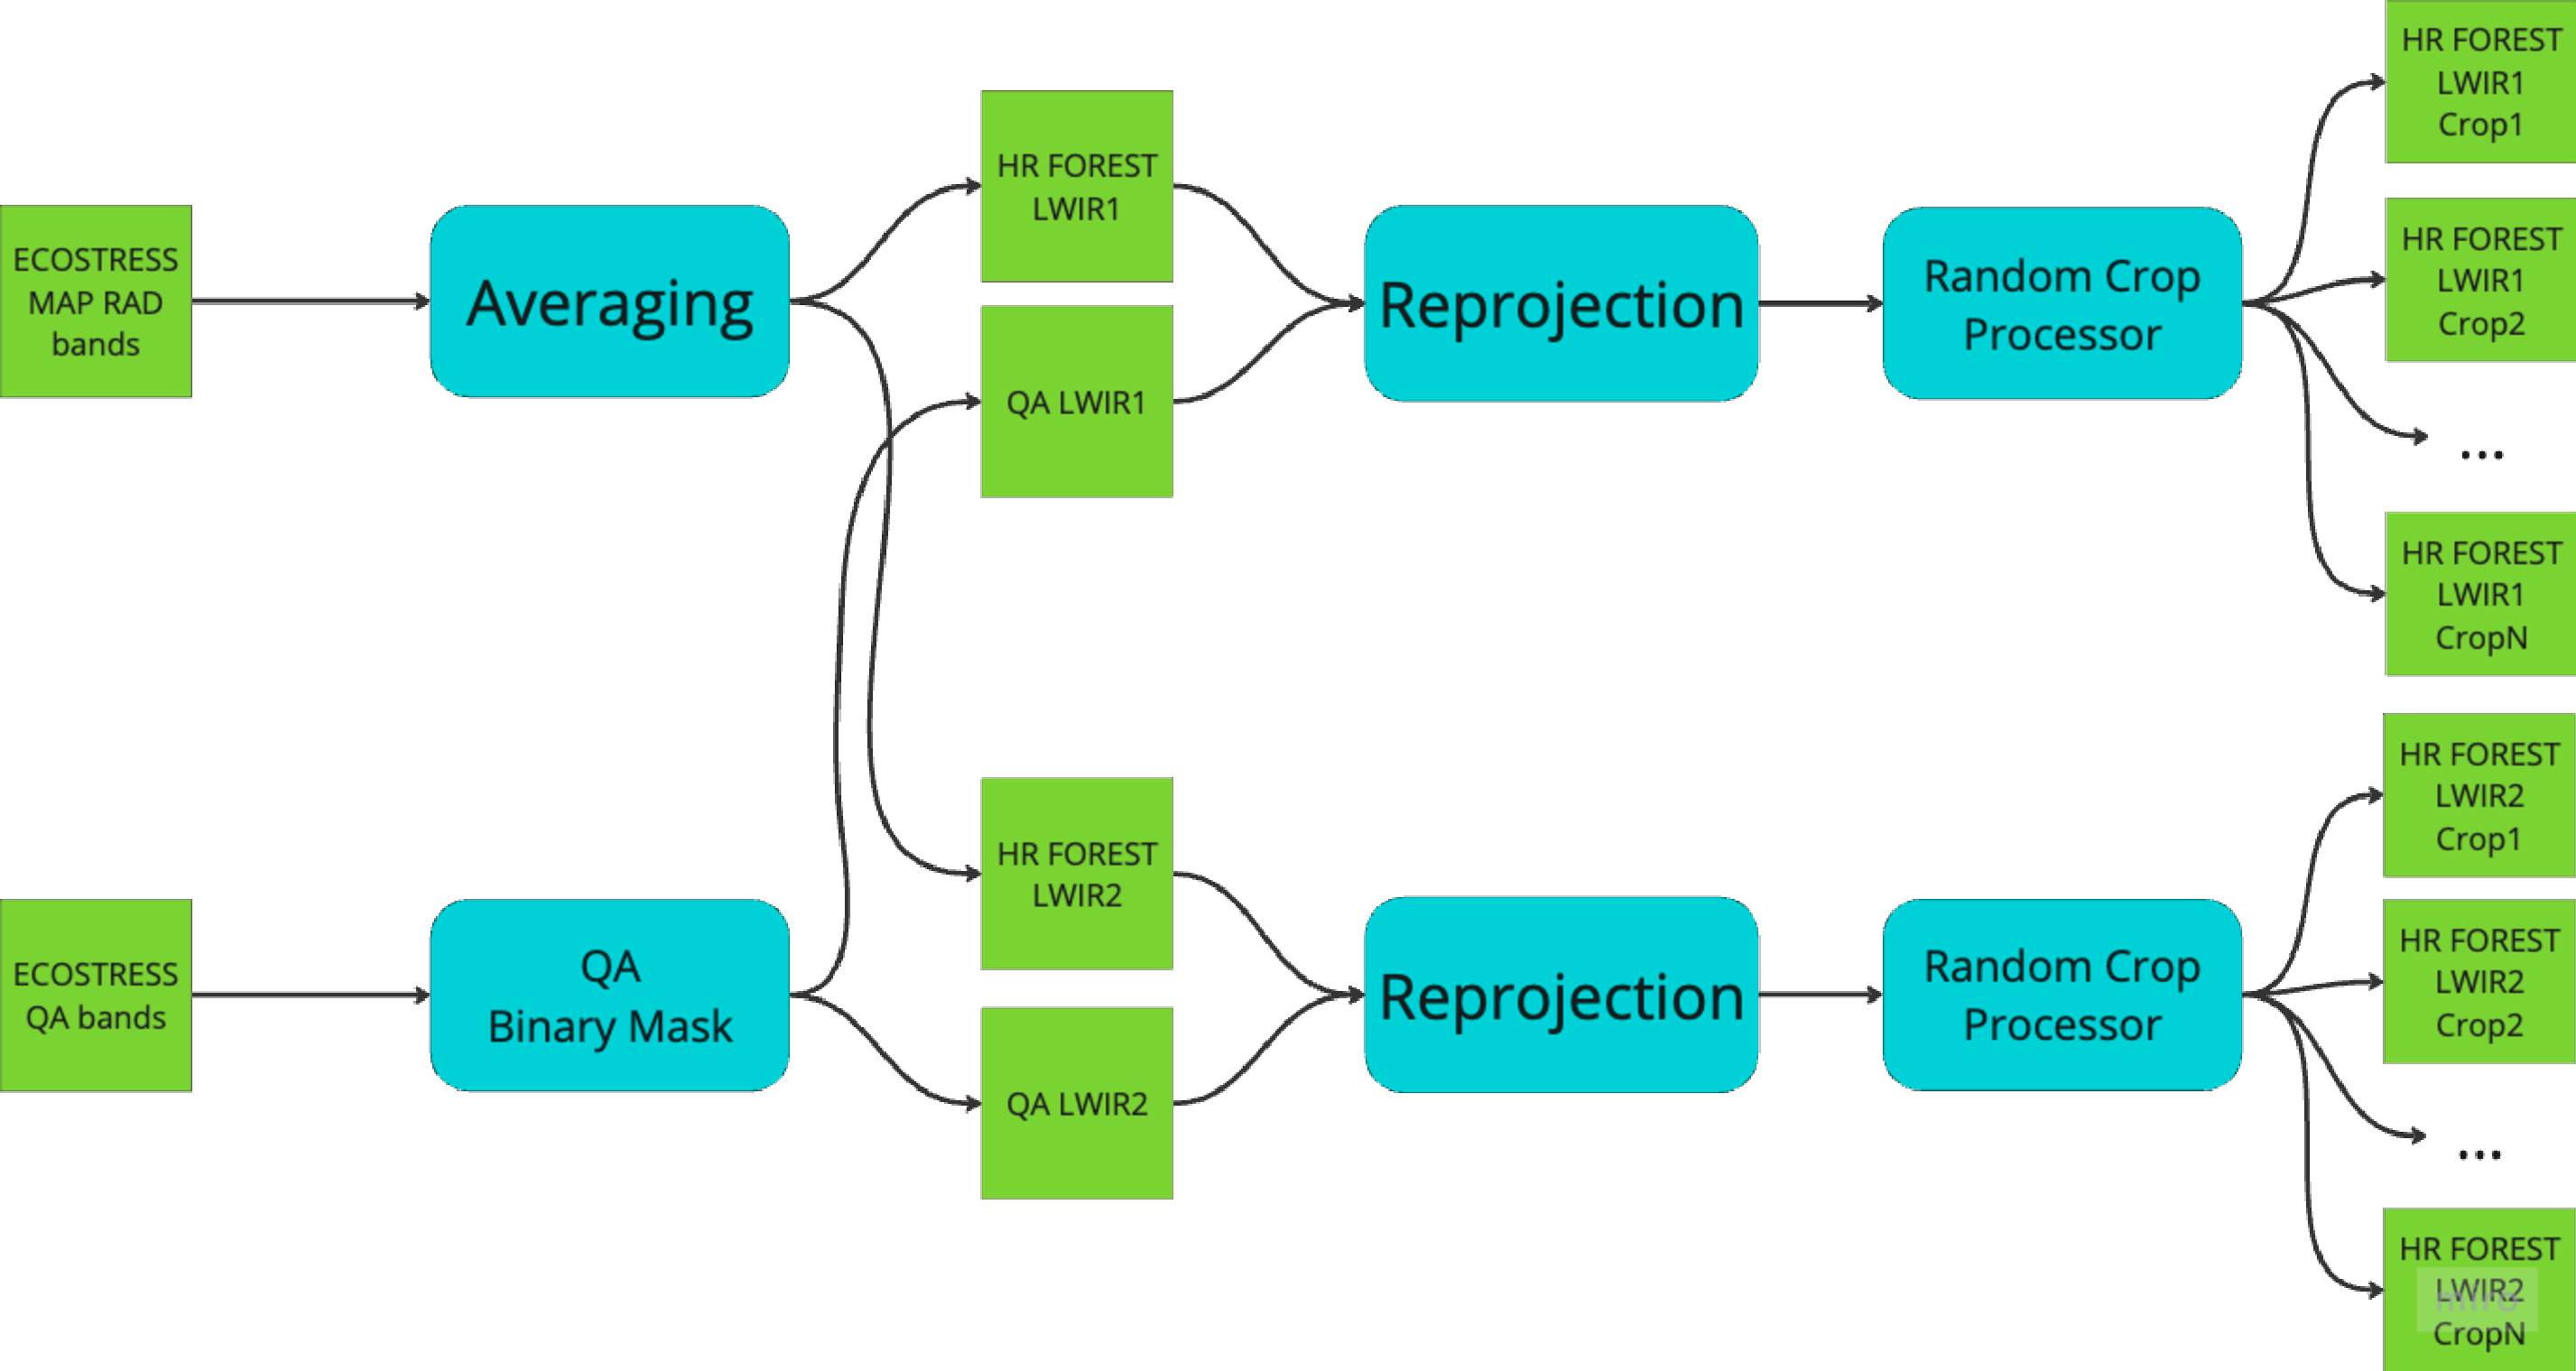
\includegraphics[width=\linewidth]{Includes/5-data_processing_flow_chart.pdf}
    \caption{Data processing workflow}
    \label{fig:5-data_processing_flow_chart}
\end{figure}

\begin{figure}[H]
    \centering
    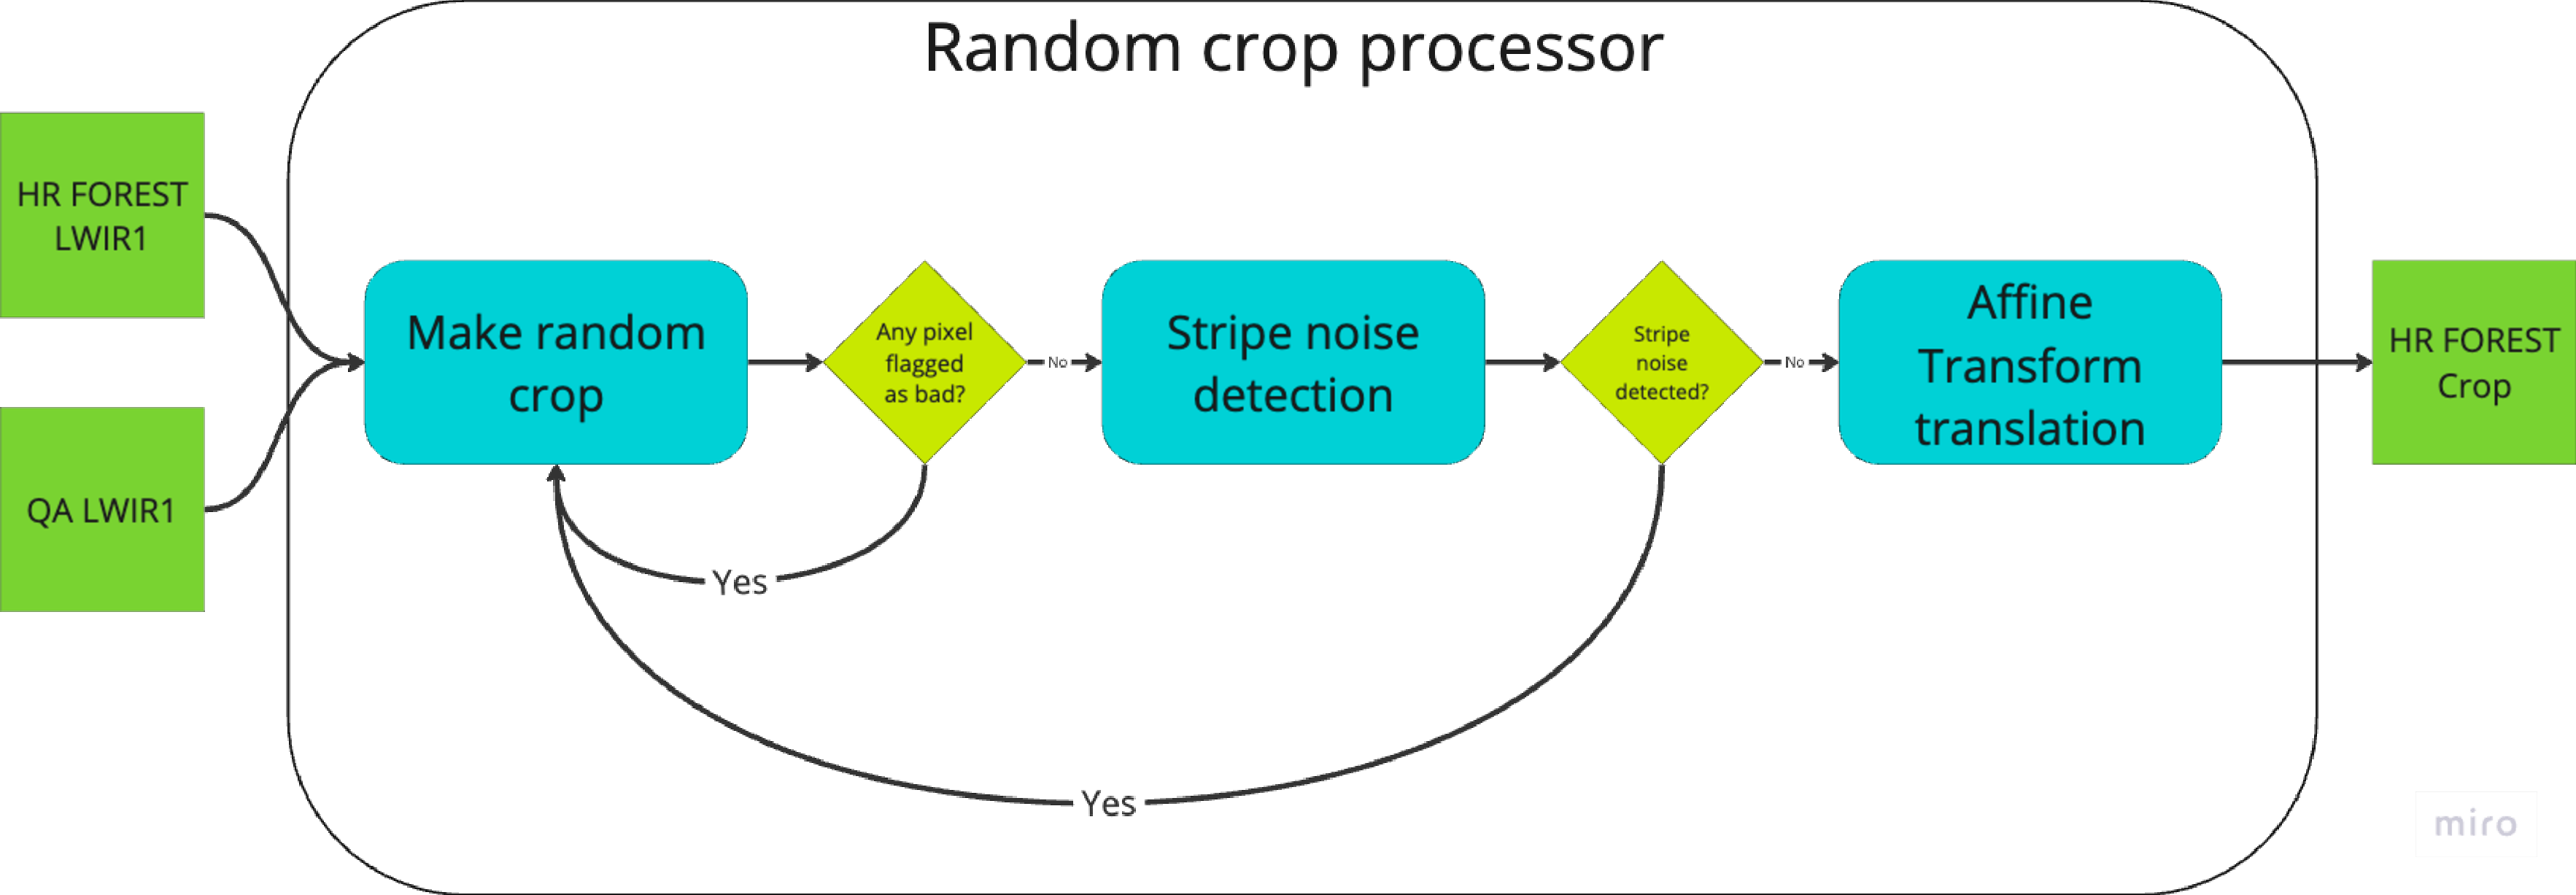
\includegraphics[width=\linewidth]{Includes/5-random_crop_processor.pdf}
    \caption{Random crop processor}
    \label{fig:5-random_crop_processor}
\end{figure}



\subsection{Obtaining FOREST-2 data}

    To obtain a dataset of FOREST-2 image, the company provides an internal API that allows the download of the scenes captured by the satellite. 
    The download of the scenes is done programmatically in the locations provided in Fig. \ref{fig:4-forest-locations}. 

    \begin{figure}[H]
        \centering
        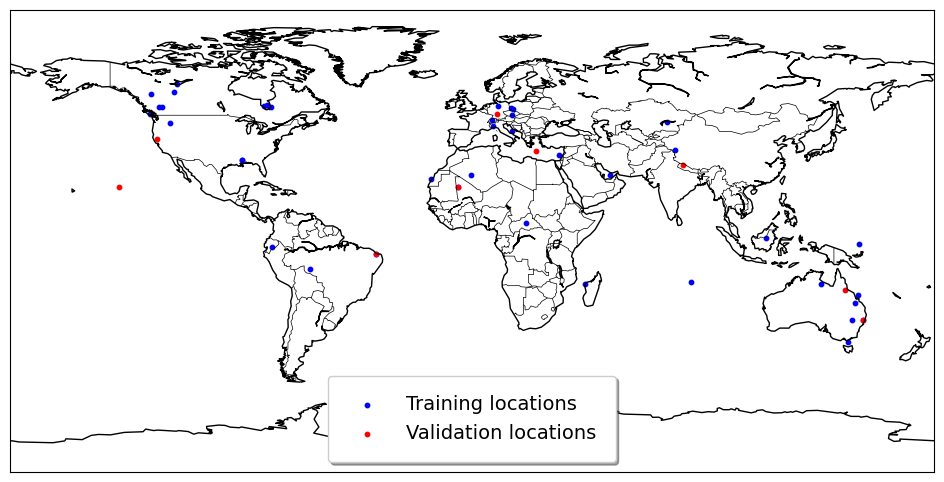
\includegraphics[width=\linewidth]{Includes/4-forest-locations.png}
        \caption{Location of the FOREST-2 scenes.}
        \label{fig:4-forest-locations}
    \end{figure}

    The scenes are downloaded in the NetCDF-4 format, containing the LWIR1, LWIR2 and MWIR bands, as long as the latitude and longitude information. 
    An example of a scene is shown in Fig. \ref{fig:4-forest-complete example}. 
    As in this work, the focus is on the long wave infrared, the MWIR band is discarded.

    \begin{figure}[H]
        \centering
        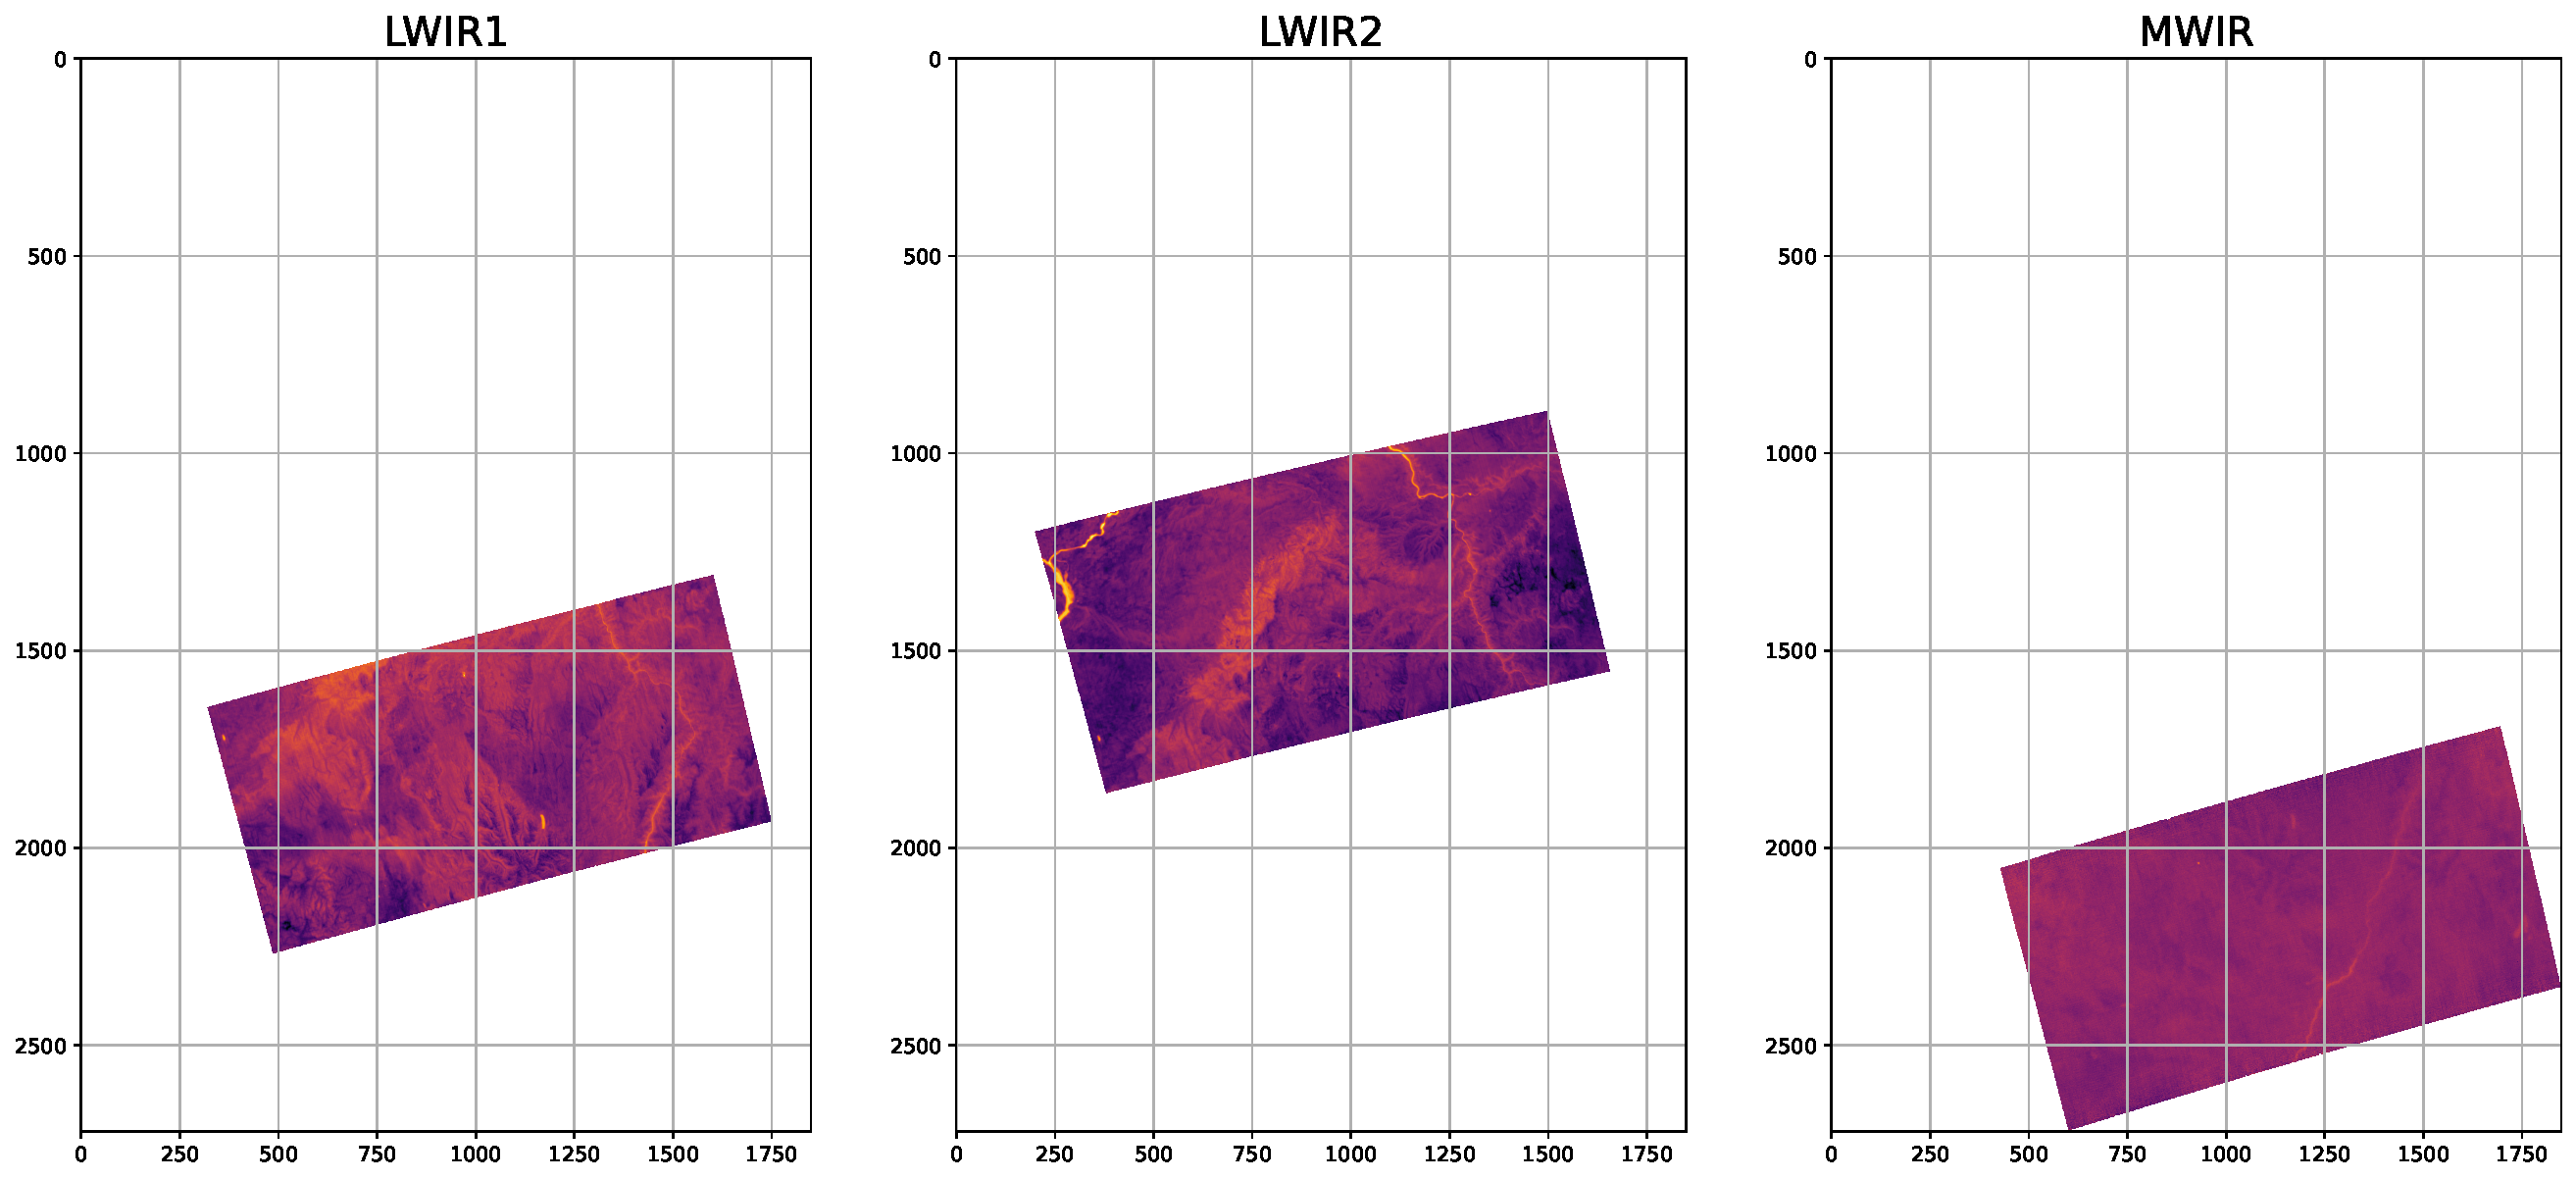
\includegraphics[width=\linewidth]{Includes/4-forest2-unprocessed-bands.pdf}
        \caption{LWIR1, LWIR2 and MWIR bands of a FOREST-2 scene downloaded from the company's API.}
        \label{fig:4-forest-complete example}
    \end{figure}

    The provided array have an enormous proportion of NA values and are not suitable for taking crops.
    For that, a bounding box is defined for each band, removing most of the NA values. 
    The resulting scenes are shown in Fig. \ref{fig:4-forest-bounding-box}.

    \begin{figure}[H]
        \centering
        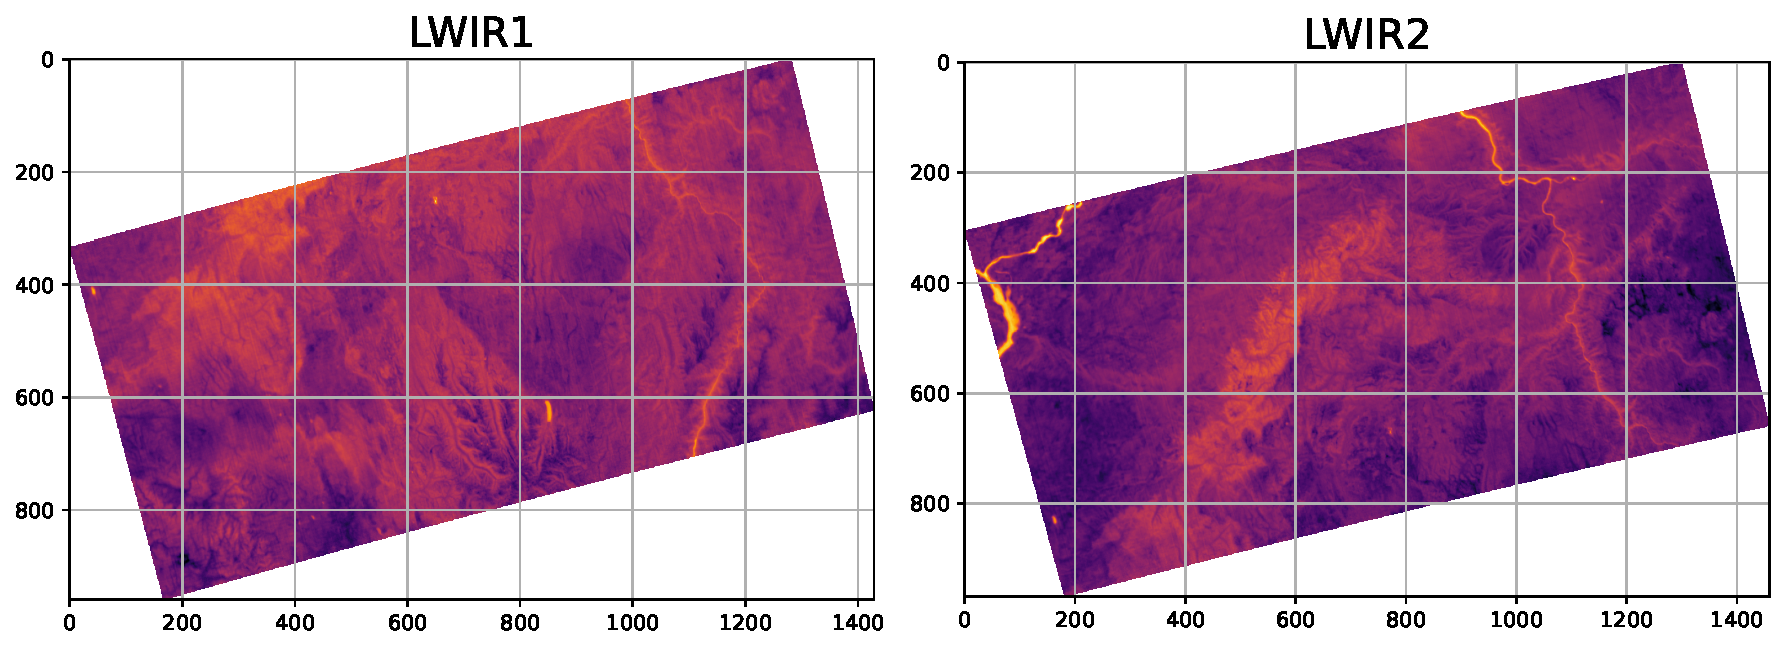
\includegraphics[width=\linewidth]{Includes/4-forest2-cropped-bands.pdf}
        \caption{LWIR1 and LWIR2 of a FOREST-2 scene downloaded from the company's API, after cropping NA values.}
        \label{fig:4-forest-bounding-box}
    \end{figure}

    A similar random crop processor as in Fig. \ref{fig:5-random_crop_processor} is employed afterwards. 
    The objective is to obtain crops 3 times less than the original size, as the objective is to train a SR model with a scale factor of 3.
    If any crop has any NA value or strip noise is detected, it is discarded and the process restarts.
    Using the latitude and the longitude information, the affine transformation is calculated so that the crops can be georeferenced, if necessary.
    
\subsection{Datasets}

For a better understanding of how the proposed architecture works, several datasets combinations are used. 
The implemented pytorch dataset class loads and yields samples from two different file locations, one for the HR images (source domain) and one for the LR images (target domain). 
The source domain are the synthetic FOREST-2 images produced from ECOSTRESS, while the target domain is composed of LR images, coming from different souces.
The samples are usually unpaired, meaning that the scenes are not compared on an image-to-image basis, but the implementation allows the use paired datasets in order to calculate supervised metrics. 
In case any of the domains has less samples than the other, the class will bootstrap it to match the size of the other.



% Please add the following required packages to your document preamble:
% \usepackage{graphicx}
\begin{table}[H]
    \centering
    \resizebox{\textwidth}{!}{%
    \begin{tabular}{c|cccc|cccc|cccc}
                & \multicolumn{4}{c|}{$\mathcal{D}_{\text{SF}-\text{SF}}$}                                                                                                                                                                                                                                           & \multicolumn{4}{c|}{$\mathcal{D}_{\text{SF}-\text{RF}}$}                                                                                                                                                                                                 & \multicolumn{4}{c|}{$\mathcal{D}_{\text{SF}-\text{RF}}^{\text{Paired}}$}                                                                                                                                                                                                      \\ \cline{2-13} 
                & \multicolumn{2}{c|}{Training}                                                                                                                                         & \multicolumn{2}{c|}{Validation}                                                                                            & \multicolumn{2}{c|}{Training}                                                                                                         & \multicolumn{2}{c|}{Validation}                                                                                  & \multicolumn{2}{c|}{Training}                                                                                                         & \multicolumn{2}{c|}{Validation}                                                                                                       \\
                & \multicolumn{1}{c|}{Source}                                                  & \multicolumn{1}{c|}{Target}                                                            & source                                                 & target                                                            & source                                                 & \multicolumn{1}{c|}{target}                                                  & source                                                 & target                                                  & source                                                 & \multicolumn{1}{c|}{target}                                                  & source                                                 & \multicolumn{1}{c|}{target}                                                  \\ \hline
    Image       & \multicolumn{1}{c|}{\begin{tabular}[c]{@{}c@{}}Synth \\ FOREST\end{tabular}} & \multicolumn{1}{c|}{\begin{tabular}[c]{@{}c@{}}Degraded\\ synth\\ FOREST\end{tabular}} & \begin{tabular}[c]{@{}c@{}}Synth\\ FOREST\end{tabular} & \begin{tabular}[c]{@{}c@{}}Degraded\\ synth\\ FOREST\end{tabular} & \begin{tabular}[c]{@{}c@{}}Synth\\ FOREST\end{tabular} & \multicolumn{1}{c|}{\begin{tabular}[c]{@{}c@{}}Real\\ FOREST-2\end{tabular}} & \begin{tabular}[c]{@{}c@{}}Synth\\ FOREST\end{tabular} & \begin{tabular}[c]{@{}c@{}}Real\\ FOREST-2\end{tabular} & \begin{tabular}[c]{@{}c@{}}Synth\\ FOREST\end{tabular} & \multicolumn{1}{c|}{\begin{tabular}[c]{@{}c@{}}Real\\ FOREST-2\end{tabular}} & \begin{tabular}[c]{@{}c@{}}Synth\\ FOREST\end{tabular} & \multicolumn{1}{c|}{\begin{tabular}[c]{@{}c@{}}Real\\ FOREST-2\end{tabular}} \\ \hline
    n           & \multicolumn{1}{c|}{13764}                                                   & \multicolumn{1}{c|}{13764}                                                             & 2676                                                   & 2676                                                              & 13764                                                  & \multicolumn{1}{c|}{4000}                                                    & 2676                                                   & 1200                                                    & 13764                                                  & \multicolumn{1}{c|}{4000}                                                    & ??                                                     & \multicolumn{1}{c|}{??}                                                      \\ \hline
    scale ratio & \multicolumn{1}{c|}{x3}                                                      & \multicolumn{1}{c|}{x3}                                                                & x3                                                     & x3                                                                & x3                                                     & \multicolumn{1}{c|}{x3}                                                      & x3                                                     & x3                                                      & x3                                                     & \multicolumn{1}{c|}{x3}                                                      & x3                                                     & \multicolumn{1}{c|}{x3}                                                      \\ \hline
    crop size   & \multicolumn{1}{c|}{264}                                                     & \multicolumn{1}{c|}{88}                                                                & 264                                                    & 88                                                                & 264                                                    & \multicolumn{1}{c|}{88}                                                      & 792                                                    & 264                                                     & 264                                                    & \multicolumn{1}{c|}{88}                                                      & ??                                                     & \multicolumn{1}{c|}{??}                                                      \\ \hline
    Paired?     & \multicolumn{2}{c|}{No}                                                                                                                                               & \multicolumn{2}{c|}{Yes}                                                                                                   & \multicolumn{2}{c|}{No}                                                                                                               & \multicolumn{2}{c|}{No}                                                                                          & \multicolumn{2}{c|}{No}                                                                                                               & \multicolumn{2}{c}{Yes}                                                                                                               \\ \hline
                & \multicolumn{1}{c|}{}                                                        & \multicolumn{1}{c|}{}                                                                  &                                                        &                                                                   &                                                        & \multicolumn{1}{c|}{}                                                        &                                                        &                                                         &                                                        & \multicolumn{1}{c|}{}                                                        &                                                        & \multicolumn{1}{c|}{}                                                        \\ \hline
                & \multicolumn{1}{c|}{}                                                        & \multicolumn{1}{c|}{}                                                                  &                                                        &                                                                   &                                                        & \multicolumn{1}{c|}{}                                                        &                                                        &                                                         &                                                        & \multicolumn{1}{c|}{}                                                        &                                                        & \multicolumn{1}{c|}{}                                                        \\ \hline
                & \multicolumn{1}{c|}{}                                                        & \multicolumn{1}{c|}{}                                                                  &                                                        &                                                                   &                                                        & \multicolumn{1}{c|}{}                                                        &                                                        &                                                         &                                                        & \multicolumn{1}{c|}{}                                                        &                                                        & \multicolumn{1}{c|}{}                                                        \\ \hline
                & \multicolumn{1}{c|}{}                                                        & \multicolumn{1}{c|}{}                                                                  &                                                        &                                                                   &                                                        & \multicolumn{1}{c|}{}                                                        &                                                        &                                                         &                                                        & \multicolumn{1}{c|}{}                                                        &                                                        & \multicolumn{1}{c|}{}                                                        \\ \hline
                & \multicolumn{1}{c|}{}                                                        & \multicolumn{1}{c|}{}                                                                  &                                                        &                                                                   &                                                        & \multicolumn{1}{c|}{}                                                        &                                                        &                                                         &                                                        & \multicolumn{1}{c|}{}                                                        &                                                        & \multicolumn{1}{c|}{}                                                       
    \end{tabular}%
    }
    \caption{}
    \label{tab:my-table}
    \end{table}


\subsubsection{Synthetic FOREST - Degraded Synthetic FOREST}
    The dataset $\mathcal{D}_{\text{SF}-\text{SF}}$ is built by taking the HR synthetic FOREST crops and applying the baseline degradation model proposed in \ref{subsec:baseline_degradation_model}. 
    The 264x264 crops are reduced to 88x88. The training set is used to train the SR Resnet model, while the validation set is used to monitor the training process and avoid overfitting. 
    Even though in this case the HR and LR version of the same scene is available, the training dataset is unpaired by shuffling the samples.
    The validation set is not shuffled, and thus can be used to calculate supervised metrics like PSNR and SSIM. 

    The parameters used for the degradation model are described below:

    \begin{table}[H]
        \centering
        \begin{tabular}{l|l}
        Parameter & Value \\ \hline
        Scale ratio & x3 \\ 
        Gaussian Kernel size & 21 \\ 
        Gaussian kernel sigma in X axis &  $\sim \mathcal{N}(1,0.3)$  \\ 
        Gaussian kernel sigma in Y axis &  $\sim \mathcal{N}(1,0.3)$  \\ 
        target radiometric error & 1.5K \\ 
        white noise factor & 0.5 \\ 
        constant noise factor & 0.5 \\ 
        \end{tabular}
        \caption{Parameters used in the degradation model employed to generate the $\mathcal{D}_{\text{SF}-\text{SF}}$ dataset.}
        \label{tab:degradation_model_parameters}
    \end{table}

\subsubsection{Synthetic FOREST - real FOREST (Unpaired)}
    The dataset $\mathcal{D}_{\text{SF}-\text{RF}}$ is composed of the 264x264 HR synthetic FOREST-2 crops as the source domain and  88x88 real FOREST-2 crops as the target domain. 
    Unfortunately, the validation dataset is not paired, as the HR and LR images are completely different scenes.
    Thus, supervised metrics are not available for the super resolved target domain images is not available. 
    The metric used to determine the best model is the PSNR from the super resolution of the output of the GAN's generator.

\subsubsection{Synthetic FOREST- real FOREST ( Paired)}
    While the training dataset is the same as in the previous case, the validation dataset is composed of a limited amount paired scenes between ECOSTRESS and FOREST are available.
    This samples allow the calculation of supervised metrics like PSNR and SSIM. 
    As supervised metrics to compare the real FOREST-2 SR with the ground truth is now available, the PSNR is used to determine the best model.




\newpage